
\documentclass[11pt]{article}
\usepackage[letterpaper,margin=0.88in,headheight=15pt]{geometry}
\usepackage[T1]{fontenc}
\usepackage{lmodern}
\usepackage{microtype}
\usepackage{amsmath,amssymb,amsthm,mathtools}
\usepackage{enumitem}
\usepackage{booktabs,longtable,array}
\usepackage{fancyhdr}
\usepackage{pdfpages}
\usepackage[hidelinks,bookmarksopen=true]{hyperref}
\usepackage{xurl}
\usepackage{xcolor}
\usepackage{tikz}
\usetikzlibrary{arrows.meta,positioning,fit,calc}
\usepackage{needspace}

\hypersetup{
  pdftitle={Depths of Induction and Formalized Self-Awareness, Version 49},
  pdfauthor={Brian Tenneson},
  pdfsubject={Version 49: clocked simulation degrees, generalized board games, proof horizons, and strategic settlement},
  pdfkeywords={induction, automated theorem proving, AMLD, generalized board games, simulation degrees, proof horizon, strategic settlement, Hilbert navigation}
}

\pagestyle{fancy}
\fancyhf{}
\lhead{Depths of Induction and Formalized Self-Awareness}
\rhead{Tenneson, Version 49}
\cfoot{\thepage}
\renewcommand{\headrulewidth}{0.4pt}

\newtheorem{definition}{Definition}[section]
\newtheorem{theorem}[definition]{Theorem}
\newtheorem{proposition}[definition]{Proposition}
\newtheorem{corollary}[definition]{Corollary}
\newtheorem{lemma}[definition]{Lemma}
\newtheorem{problem}[definition]{Open Problem}
\theoremstyle{remark}
\newtheorem{remark}[definition]{Remark}
\newtheorem{example}[definition]{Example}
\newtheorem{question}[definition]{Research Question}

\newcommand{\N}{\mathbb N}
\newcommand{\Npos}{\mathbb N^{+}}
\newcommand{\Con}{\operatorname{Con}}
\newcommand{\Succ}{\operatorname{Succ}}
\newcommand{\dom}{\operatorname{dom}}
\newcommand{\dist}{\operatorname{dist}}
\newcommand{\Reach}{\operatorname{Reach}}
\newcommand{\Bank}{\mathsf{BANK}}
\newcommand{\calG}{\mathcal G}
\newcommand{\calS}{\mathcal S}
\newcommand{\calA}{\mathcal A}
\newcommand{\calT}{\mathcal T}
\newcommand{\calW}{\mathcal W}
\newcommand{\infstep}{\ell_{\mathrm{inf}}}
\newcommand{\Dclk}{\mathcal D_{\mathrm{clk}}}
\newcommand{\preclk}{\preceq_{\mathrm{clk}}}
\newcommand{\simclk}{\sim_{\mathrm{clk}}}
\newcommand{\Obs}{\operatorname{Obs}}
\newcommand{\depthsurl}{https://btenneson.github.io/pub/cs.LO_Logic_in_Computer_Science/depths_of_induction_v48/}
\newcommand{\gbgurl}{https://btenneson.github.io/pub/cs.LO_Logic_in_Computer_Science/generalized_board_games_tic_tac_toe_chess_001/}
\newcommand{\hilberturl}{https://btenneson.github.io/pub/cs.LO_Logic_in_Computer_Science/from_theoremhood_as_reachability_to_hilbert_addressed_inference_spaces_003/}

\newcommand{\vfortynineoverlay}{%
  \thispagestyle{empty}%
  \begin{tikzpicture}[remember picture,overlay]
    \fill[white] (current page.north west) rectangle ([yshift=-0.56in]current page.north east);
    \draw[line width=0.35pt] ([xshift=0.55in,yshift=-0.51in]current page.north west) --
      ([xshift=-0.55in,yshift=-0.51in]current page.north east);
    \node[anchor=north west,font=\scriptsize] at
      ([xshift=0.55in,yshift=-0.16in]current page.north west)
      {Depths of Induction and Formalized Self-Awareness};
    \node[anchor=north east,font=\scriptsize] at
      ([xshift=-0.55in,yshift=-0.16in]current page.north east)
      {Version 49 retained Version 48 core};
    \node[anchor=south,font=\tiny,text=gray!80!black] at
      ([yshift=0.13in]current page.south)
      {Retained Version 48 core; the editable Version 49 integrations following it state the new claims of this edition.};
  \end{tikzpicture}%
}

\begin{document}
\hypersetup{pageanchor=false}
\pagenumbering{roman}

\begin{titlepage}
\thispagestyle{empty}
\centering
\vspace*{0.65in}
{\Huge\bfseries Depths of Induction and\\[0.12em]Formalized Self-Awareness\par}
\vspace{0.32in}
{\LARGE\bfseries Version 49\par}
\vspace{0.28in}
{\Large Generalized Board Games, Strategic Horizons,\\
and Clocked Simulation Degrees\par}
\vspace{0.8in}
{\Large Brian Tenneson\par}
\vspace{0.16in}
{\large September 24, 2026\par}
\vfill
\begin{minipage}{0.82\textwidth}
\small
\textbf{Scope freeze.}
Version 49 retains the Version 48 core and closes the present development cycle by integrating:
(1) the settled order theory of clocked simulation degrees;
(2) generalized-board-game operationalizations of proof and search;
(3) the separation of proof, discovery, and forced-settlement horizons;
(4) a GBG interpretation of scheduled simulation degrees; and
(5) a Hilbert-addressed ATP case study.
Later themes belong to a subsequent edition rather than being allowed to make Version 49 a moving target.
\end{minipage}
\vfill
\end{titlepage}

\begin{abstract}
Version 49 retains the mathematical core of Version 48 and integrates two later developments.
First, the clocked-simulation preorder on semi-ideal computers is sharpened through its quotient degree order:
the degree poset contains a countably infinite antichain of finite, finitely describable machines,
fails to be a lattice even when relevant common bounds exist,
admits synchronized dynamic invariants, and retains these phenomena under effective simulation.
Because only countably many finite descriptions exist, the countably infinite antichain has the largest
possible cardinality among antichains restricted to finitely describable machines.

Second, generalized board games (GBGs) supply an operational state-transition interpretation of
formal inference, ATP search, and cooperative AMLD settlement.
Finitary inference can be lifted to unary moves on complete derivation states;
theoremhood becomes finite target-region reachability;
an inference-step proof horizon becomes directed distance;
and future-complete operational states admit transposition quotienting.
The resulting geometry separates intrinsic proof horizon, implementation-dependent discovery effort,
and a strategic or scheduler-robust forced-settlement horizon.
Conservative BANK growth can shorten certified routes without changing consequence closure.

The final integration defines a scheduled/deterministic GBG simulation-degree viewpoint and uses
the Hilbert-addressed inference-space architecture as a case study.
Different schedulers may preserve theoremhood and proof depth while inducing different operational
chronologies; whether particular schedulers occupy the same or distinct clocked degrees is posed as a
precise comparison problem rather than assumed.
\end{abstract}

\section*{Version 49 integration map}
\addcontentsline{toc}{section}{Version 49 integration map}
\begin{longtable}{p{0.23\textwidth}p{0.68\textwidth}}
\toprule
\textbf{Component} & \textbf{Version 49 status}\\
\midrule
Retained Version 48 core &
Preserved as the documentary mathematical baseline, with Version 49 running identification.\\
Clocked simulation degrees &
Settlements of former Open Problems 9.1, 9.3, 9.4, and 9.5 integrated as proved results.\\
Former Open Problem 9.2 &
Greatest-degree question remains open in this edition.\\
Generalized board games &
Used as an operationalization of finitary proof and search states, not merely as analogy.\\
Strategic horizons &
Proof horizon, discovery effort, and forced/scheduler-robust settlement horizon are separated.\\
AMLD/BANK &
Nonstarvation is treated as an admissibility restriction on external scheduling; BANK growth as conservative road-building.\\
GBG simulation degrees &
The old clocked-simulation preorder is reinterpreted for deterministic scheduled GBG chronologies.\\
Hilbert case study &
Hilbert-, lexicographic-, random-, or learned-order search on the same action fibers becomes a concrete degree-comparison problem.\\
\bottomrule
\end{longtable}

\tableofcontents
\clearpage
\pagenumbering{arabic}

\part*{Retained Version 48 Core}
\addcontentsline{toc}{part}{Retained Version 48 Core}
The following pages retain the Version 48 core. They are carried forward as the baseline on which the
editable Version 49 integrations are built. The Version 49 additions begin immediately after the retained core.

\hypersetup{pageanchor=false}

\includepdf[
  pages={2-165},
  fitpaper=true,
  pagecommand={\vfortynineoverlay}
]{Depths_of_Induction_Version_48.pdf}
\hypersetup{pageanchor=true}
\clearpage
\part*{Version 49 Integration A: Clocked Simulation Degrees}
\addcontentsline{toc}{part}{Version 49 Integration A: Clocked Simulation Degrees}

\section{Standing clocked-simulation definitions}

Let a semi-ideal computer (SIC) be \(M=(C_M,H_M)\) with state space \(S_M\).
A \emph{clocked deterministic simulation} from \(M\) to \(N\) is a pair \((f,\rho)\) such that
\(f:S_M\to S_N\) is injective,
\(\rho:\Npos\to\Npos\) satisfies \(\rho(1)=1\), is nondecreasing and unbounded, and
for all \(p\in S_M\) and \(m\in\Npos\),
\[
f(C_M(p,m))=C_N(f(p),\rho(m)),
\qquad
H_M(p,m)=H_N(f(p),\rho(m)).
\]
Write \(M\preclk N\).
Mutual clocked simulation defines
\[
M\simclk N
\iff
M\preclk N\ \text{and}\ N\preclk M,
\]
and the quotient degree poset is
\[
\Dclk := \mathrm{SIC}/\!\simclk .
\]

Reflexivity is witnessed by identity maps and the identity clock.
Transitivity follows by composing injective state maps and the nondecreasing unbounded clocks.
Thus \(\preclk\) is a preorder, while the quotient relation on degrees is a partial order.

\section{Settlement of former Open Problem 9.1: infinite antichains}

The Version 48 addendum had already shown incomparable degrees, a strict chain of order type
\(\omega\), and finite antichains of arbitrarily large size.
The remaining question was whether a genuine infinite antichain exists; the settlement recorded here
follows the companion settlement note~\cite{TennesonSettlements}.

\begin{theorem}[Infinite clocked-simulation antichain]\label{thm:inf-antichain}
The poset \(\Dclk\) contains a countably infinite antichain consisting of degrees of finite,
finitely describable SICs.
\end{theorem}

\begin{proof}
Let \(\pi\in S_n\) be a finite permutation. Define
\[
Y_\pi=\{a_1,b_1,\ldots,a_n,b_n\},
\qquad
p_i=\{a_i\},
\qquad
q_i=\{a_i,b_i\},
\]
and take the full finite state space
\[
S_\pi=\mathcal P(Y_\pi).
\]
Define \(M_\pi=(C_\pi,H_\pi)\) by making every state outside the distinguished \(p_i\)'s
static and permanently unhalted, and by setting
\[
C_\pi(p_i,t)=
\begin{cases}
p_i,&t\le i,\\
q_i,&t\ge i+1,
\end{cases}
\qquad
H_\pi(p_i,t)=
\begin{cases}
0,&t<n+1+\pi(i),\\
1,&t\ge n+1+\pi(i).
\end{cases}
\]
Thus the distinguished trajectories have their unique strict growth events in the fixed order
\[
1<2<\cdots<n,
\]
while their halting thresholds occur in the relative order encoded by \(\pi\).
Every halting threshold lies after every growth threshold, so the stage-one, monotonicity,
persistent-halting, and frozen-after-halting requirements are immediate; hence \(M_\pi\) is a finite SIC.

Suppose \(M_\pi\preclk M_\sigma\) via \((f,\rho)\), where \(\sigma\in S_m\).
Because each \(p_i\) has a nonconstant trajectory and \(f\) is injective,
its image must be one of the distinguished nonconstant trajectories of \(M_\sigma\).
Write this image as \(p_{j_i}\leadsto q_{j_i}\).
Comparing two source trajectories at a common stage at which the earlier one has grown and the
later one has not, and then applying the common clock \(\rho\), forces
\[
j_1<j_2<\cdots<j_n.
\]
Likewise, comparing one halted and one unhalted source trajectory at the same source stage and using
halting preservation forces
\[
\pi(i)<\pi(k)
\iff
\sigma(j_i)<\sigma(j_k).
\]
Hence \(\pi\) occurs as a permutation pattern in \(\sigma\):
\[
M_\pi\preclk M_\sigma
\Longrightarrow
\pi\le_{\mathrm{pat}}\sigma.
\]
Finite permutations under pattern containment contain a countably infinite antichain~\cite{SpielmanBona}.
Choosing such a family \(\pi_1,\pi_2,\ldots\) gives, for \(r\ne s\),
\[
M_{\pi_r}\not\preclk M_{\pi_s},
\qquad
M_{\pi_s}\not\preclk M_{\pi_r}.
\]
Therefore the degrees \([M_{\pi_r}]_{\mathrm{clk}}\) form a countably infinite antichain.
Every \(M_{\pi_r}\) is finite and therefore finitely describable.
\end{proof}

\begin{corollary}[Cardinality-maximal width in the finitely describable class]\label{cor:max-countable}
Among finitely describable SICs, the cardinality \(\aleph_0\) achieved by
Theorem~\ref{thm:inf-antichain} is the largest possible cardinality of an antichain.
\end{corollary}

\begin{proof}
Finite descriptions over a finite or countable description alphabet form a countable set.
Hence there are at most countably many finitely describable SICs, and therefore at most countably
many clocked-simulation degrees represented by them.
Theorem~\ref{thm:inf-antichain} realizes a countably infinite antichain.
\end{proof}

\begin{remark}
``Cardinality-maximal'' here does not mean that the displayed antichain is a
\emph{maximal antichain} under inclusion.
It means only that no antichain drawn from the finitely describable class can have cardinality
strictly larger than \(\aleph_0\).
\end{remark}

\section{Settlement of former Open Problem 9.3: joins and meets}

For a finite static SIC with constant halting value in time, write \(S(h,u)\) when exactly
\(h\) states are permanently halted and \(u\) are permanently unhalted.
Because the full finite state space is a power set,
\[
h+u=2^{|Y|}.
\]
Moreover,
\[
S(h,u)\preclk S(h',u')
\iff
h\le h'\ \text{and}\ u\le u'.
\]

\begin{theorem}[Failure of lattice structure]\label{thm:nonlattice}
The poset \(\Dclk\) is not a lattice.
More strongly:
\begin{enumerate}[label=(\roman*)]
\item some two degrees have common upper bounds but no join;
\item some two degrees have common lower bounds but no meet.
\end{enumerate}
\end{theorem}

\begin{proof}
Take \(A=S(3,1)\) and \(B=S(1,3)\).
They have common upper bounds, for example \(U=S(3,5)\) and \(V=S(5,3)\).
If a join \(J\) existed, then \(J\preclk U,V\).
Since \(U,V\) are static, injective state preservation forces \(J\) itself to be static with constant
halting type, so \(J=S(h_J,u_J)\).
The lower-bound requirements \(A,B\preclk J\) force \(h_J,u_J\ge 3\),
while \(J\preclk U,V\) forces \(h_J,u_J\le 3\).
Thus \(J\) would have exactly six states, impossible because a finite SIC state space has power-of-two
cardinality.

Dually, take \(A'=S(3,5)\) and \(B'=S(5,3)\).
They have common lower bounds \(S(3,1)\) and \(S(1,3)\).
A greatest lower bound would again have to be \(S(3,3)\), which is unrealizable for the same
six-state obstruction.
\end{proof}

\section{Settlement of former Open Problem 9.4: synchronized invariants}

\begin{definition}[Finite synchronized observation spectrum]
Choose finitely many marked states \(p_1,\dots,p_r\in S_M\) and a finite nondecreasing stage sequence
\(t_1\le\cdots\le t_s\).
Record all halting bits \(H_M(p_i,t_j)\) and all equality/inequality relations among the observed states
\(C_M(p_i,t_j)\).
Let \(\Obs(M)\) be the set of all such finite patterns, up to relabeling of the marked states.
\end{definition}

\begin{theorem}[Dynamic monotonicity and complete static invariant]\label{thm:obs}
If \(M\preclk N\), then
\[
\Obs(M)\subseteq\Obs(N).
\]
Hence \(\Obs\) is a monotone dynamic invariant.
On the finite static constant-halting subclass, the pair \((h,u)\) is a complete invariant of
clocked-simulation degree.
\end{theorem}

\begin{proof}
If \((f,\rho)\) witnesses \(M\preclk N\), use the target marked states
\(f(p_1),\dots,f(p_r)\) and target stages
\(\rho(t_1)\le\cdots\le\rho(t_s)\).
The simulation equations preserve all recorded halting bits.
Injectivity preserves equality and inequality exactly.
Thus every synchronized finite pattern realized in \(M\) is realized in \(N\).

For finite static constant-halting SICs,
\[
S(h,u)\preclk S(h',u')
\iff
h\le h'\ \text{and}\ u\le u'.
\]
Mutual simulation therefore holds exactly when \((h,u)=(h',u')\).
\end{proof}

\section{Settlement of former Open Problem 9.5: effective degrees}

\begin{theorem}[Effective survival theorem]\label{thm:effective-survival}
Under effective clocked simulation, all of the following already occur among finite effectively
presented SICs:
\begin{enumerate}[label=(\roman*)]
\item incomparable degrees;
\item absence of a least degree;
\item a strict chain of order type \(\omega\);
\item finite antichains of arbitrarily large size;
\item a countably infinite antichain;
\item failure of joins and meets as in Theorem~\ref{thm:nonlattice}.
\end{enumerate}
\end{theorem}

\begin{proof}
Every finite SIC has an effective presentation by enumerating its finite state set.
Its coded stage and halting maps are finite lookup functions.
Every positive witness used in the finite constructions can be chosen as an explicit finite injection
with the identity clock and is computable.
Every negative result rules out an ordinary clocked simulation and therefore also rules out an
effective one.
The infinite antichain of Theorem~\ref{thm:inf-antichain} consists entirely of finite machines,
so the same family is an antichain for effective clocked simulation.
\end{proof}

\section{The one former open problem intentionally left open}

\begin{problem}[Greatest clocked-simulation degree]\label{prob:greatest}
Does \(\Dclk\) have a greatest element?
\end{problem}

Version 49 does not infer a negative answer merely from the failure of natural universal-looking
candidates.
The greatest-degree question remains separate from the infinite-antichain and nonlattice results.

\clearpage
\part*{Version 49 Integration B: Generalized Board Games and Strategic Settlement}
\addcontentsline{toc}{part}{Version 49 Integration B: Generalized Board Games and Strategic Settlement}


\section{Purpose of the synthesis}

Two papers in the same formal program approach proof from opposite directions. \emph{Depths of Induction}, Version 48 (hereafter \emph{Depths v48})~\cite{TennesonDepths48} starts with general formal systems and develops inference closure, proof horizons, proof search, machine learning guidance, cooperative AMLDs, typed verified memory, and formalized self-awareness. The GBG paper~\cite{TennesonGBG} starts with familiar games and shows that their rule-complete states and legal moves instantiate the same $xyz$ architecture.

The important interaction is not the analogy ``proofs are like games.'' That observation is too weak. The useful question is whether the GBG construction supplies additional mathematical structure for the objects already present in \emph{Depths v48}. The answer developed here is yes, but at three different levels that must not be conflated:
\begin{enumerate}[label=\textbf{L\arabic*.},leftmargin=3.2em]
\item \textbf{Logical derivation level.} A finitary proof system can be lifted to a unary transition graph on finite derivation states. Theoremhood becomes reachability and a step-count proof horizon becomes graph distance.
\item \textbf{Operational search level.} A concrete ATP has richer states: queues, open goals, scores, candidate caps, seeds, BANK snapshots, and other implementation data. Discovery cost is a hitting time in this operational graph, not a synonym for proof length.
\item \textbf{Strategic control level.} When some transitions are selected by a controller and others by a scheduler, opponent, environment, or cooperating role, ordinary reachability may be strengthened to forced reachability. This gives a robust or forced-settlement horizon with min/max recurrences.
\end{enumerate}

The third level is the genuinely new conceptual layer for \emph{Depths v48}. Version 48 already proves a nonstarvation-based emulation result. The GBG viewpoint reveals that theorem as a constrained forced-reachability statement.

\section{Standing formal framework from Depths v48}

\subsection{Formal systems and partial inference rules}

Fix an $xyz$ formal system
\[
F=(x,y,z),
\]
where $x$ is a nonempty alphabet, $y$ is a set of well-formed finite strings over $x$, and each $r\in z$ is a finitary partial rule
\[
r:y^k\rightharpoonup y
\]
for some positive finite arity $k$. Partiality represents applicability: an inference rule need not be legal on every $k$-tuple.

For a premise set $B\subseteq y$, write
\[
B\vdash_F\varphi,
\qquad
\Con_F(B)=\{\varphi\in y:B\vdash_F\varphi\}.
\]
The Version 48 proof-horizon notation for a provable object-level target is
\[
\|\varphi\|_F(B)
=
\min\{\,|\pi|:\pi\text{ is an }F\text{-proof of }\varphi\text{ from }B\,\},
\]
with value $\infty$ if no proof exists. Because proof-length conventions differ, we shall also use a cost that counts primitive inference applications explicitly.

\begin{definition}[Inference-step proof cost]
For a finite proof $\pi$ from $B$, let $\infstep(\pi)$ be the number of non-premise primitive inference applications appearing in $\pi$. Define
\[
H_F^{\mathrm{inf}}(B,\varphi)
:=
\min\{\infstep(\pi):\pi\text{ proves }\varphi\text{ from }B\},
\]
with value $\infty$ if no proof exists.
\end{definition}

This auxiliary convention is chosen because one legal state transition below will correspond to one primitive inference application. If the Version 48 symbol $|\pi|$ is instantiated by the same convention, then $H_F^{\mathrm{inf}}=\|\cdot\|_F$. Under a line-count convention the quantities differ by the declared accounting of premises and repeated lines.

\subsection{The Version 48 separation of metrics}

A central discipline of \emph{Depths v48} is that proof length, logical birth stage, expansion count, wall-clock time, and total work are different quantities. In particular, Version 48 defines an expansion discovery cost $\widetilde E_M(\varphi)$ for a fixed ATP trajectory and records right-censored failure at budget $B$ as $\widetilde E_M(\varphi)>B$, not as an exact value.

That distinction will become geometric:
\begin{center}
\begin{tabular}{p{0.27\textwidth}p{0.62\textwidth}}
\toprule
\textbf{Quantity} & \textbf{GBG interpretation}\\
\midrule
Intrinsic proof horizon & Shortest directed path in a logical derivation-state graph.\\
Discovery expansions & Hitting time along one implementation-dependent search trajectory or search tree.\\
Wall-clock time & A cost placed on operational transitions and resource contention.\\
Total work & Aggregate cost over all participating channels, verification, and BANK management.\\
Forced-settlement horizon & Worst-case compatible path length under a controller strategy and admissible external choices.\\
\bottomrule
\end{tabular}
\end{center}

\section{The GBG layer}

The GBG paper specializes the $xyz$ formalism to systems in which every well-formed object is a rule-complete game state and every inference rule is a partial unary move rule
\[
r_\mu:y\rightharpoonup y.
\]
A distinguished initial state $s_0$ acts as a hypothesis, and the paper proves
\[
s\in\Con_F(\{s_0\})
\iff
s\text{ is reachable from }s_0\text{ by finitely many legal moves}.
\]
It also distinguishes the match tree of histories from the state graph of endpoints and develops alternating forced-win regions. The forced-win horizon satisfies a minimum recursion on the favored player's turns and a maximum recursion on the opponent's turns.

The apparent mismatch with \emph{Depths v48} is that general inference rules may be $k$-ary while GBG move rules are unary. The first task is therefore to lift $k$-ary inference into unary transitions on a richer state space.

\section{Operational lifting: from \texorpdfstring{$k$}{k}-ary inference to unary proof-state moves}

\begin{definition}[Finite derivation state]
Fix $F=(x,y,z)$ and a finite initial premise sequence $B_0=(\beta_1,\ldots,\beta_m)$. A finite derivation state is a finite sequence
\[
S=(\beta_1,\ldots,\beta_m,\varphi_{m+1},\ldots,\varphi_n)
\]
such that every $\varphi_j$ with $j>m$ is the conclusion of one legal primitive inference from formulas occurring earlier in the sequence.
\end{definition}

The use of a sequence rather than a set preserves enough information to reconstruct a certificate. If only future logical applicability matters, one may later quotient away redundant history.

For every primitive rule $r:y^k\rightharpoonup y$ and every ordered index tuple $\mathbf i=(i_1,\ldots,i_k)$, define a partial unary operator on derivation states by
\[
\widehat r_{\mathbf i}(S)
=
S^\frown r(\varphi_{i_1},\ldots,\varphi_{i_k})
\]
whenever all indices refer to entries already in $S$ and the tuple lies in $\dom(r)$. Otherwise the operator is undefined.

\begin{theorem}[Operational lifting theorem]
Let $F$ be a finitary $xyz$ formal system and $B_0$ a finite premise sequence. There is a unary state-transition system
\[
\calG_{\mathrm{der}}(F,B_0)
\]
whose states are finite legal derivation states and whose legal transitions append exactly one primitive inference conclusion, such that finite $F$-proofs from $B_0$ are in canonical correspondence with finite paths beginning at the initial state $S_0=B_0$, up to inessential choices concerning unused or repeated proof lines.
\end{theorem}

\begin{proof}
Given a proof, read its primitive inference lines in proof order and append each conclusion to the current derivation state. Every append is legal because its premises occur earlier and the underlying rule is defined on that premise tuple. Conversely, a finite path in the transition system records, at every edge, a primitive rule and the earlier entries used as premises. Reading those labels recovers a finite derivation. Unused or deliberately repeated lines may create different derivation-state histories with the same essential proof dependency DAG; this is the stated inessential freedom.
\end{proof}

\begin{corollary}[Theoremhood as target-region reachability]
For $T\in y$, define
\[
W_T:=\{S:T\text{ occurs in }S\}.
\]
Then
\[
B_0\vdash_F T
\iff
W_T\cap\Reach(S_0)\ne\varnothing.
\]
\end{corollary}

\begin{proof}
A proof of $T$ lifts to a path whose final state contains $T$. Conversely, a reachable state containing $T$ contains a recorded legal derivation of $T$ from $B_0$.
\end{proof}

\subsection{What has and has not been shown}

The operational lifting does not say that every formal system is literally a competitive board game. It says that its finite derivations admit a GBG-style unary state-transition presentation. Competition, alternating control, and forced winning are additional structure. This separation will matter later.

\section{Proof horizon as directed distance}

Give every derivation-state edge unit cost. For a state $S$ and target region $W$, define the directed graph distance
\[
\dist_{\calG}(S,W)
=
\inf\{n:\text{there is an }n\text{-edge path from }S\text{ to }W\},
\]
with value $\infty$ when no such path exists.

\begin{theorem}[Proof-horizon/distance theorem]
Under the inference-step cost convention,
\[
\boxed{
H_F^{\mathrm{inf}}(B_0,T)
=
\dist_{\calG_{\mathrm{der}}(F,B_0)}(S_0,W_T).
}
\]
\end{theorem}

\begin{proof}
By the operational lifting theorem, every proof with $n$ primitive inference applications gives an $n$-edge path to $W_T$, and every $n$-edge path to $W_T$ gives a proof using $n$ primitive inference applications. Taking minima on the two corresponding sets gives equality.
\end{proof}

\begin{remark}[Line-count conventions]
If proof length counts premise lines, displayed lines, or administrative certificate material, exact equality should not be asserted without reconciling cost conventions. The geometric theorem is exact for the edge cost explicitly defined above.
\end{remark}

This gives a precise version of the slogan
\[
\boxed{\text{proof horizon}=\text{distance to a target region}}
\]
without importing any Euclidean or Hilbert-coordinate geometry. It is intrinsic directed graph distance in the derivation transition system.

\section{Histories, states, and transpositions}

The GBG paper~\cite{TennesonGBG} distinguishes a match tree from its endpoint state graph. The same distinction is essential in proof search.

\begin{definition}[Derivation history tree]
The derivation history tree $\calT(S_0)$ has as its depth-$n$ nodes the move-labeled legal derivation histories of exactly $n$ primitive inference transitions beginning at $S_0$.
\end{definition}

Two different histories can establish the same collection of usable formulas. Whether they can be safely merged depends on what future transitions are allowed to inspect.

\begin{definition}[Future-complete equivalence]
Fix an observation-label map $L$ on operational states that records every state predicate relevant to the claims under study---at minimum target membership, settlement status, and verifier/acceptance status when those notions are present. Two operational states $S$ and $S'$ are future-complete equivalent, written $S\equiv_{\mathrm{fc}}S'$, if they are related by a label-preserving strong bisimulation: $L(S)=L(S')$, and for every labeled transition $S\xrightarrow{a}T$ there is a transition $S'\xrightarrow{a}T'$ with $T\equiv_{\mathrm{fc}}T'$, and conversely for every transition from $S'$.
\end{definition}

For pure monotone logical derivation, a simpler sufficient condition is often equality of the available formula set, provided candidate generation depends only on that set and the fixed target/environment. For a concrete ATP, the rule-complete state may need to include queues, open goals, declaration cutoffs, caches, scores, seeds, and BANK snapshots.

\begin{proposition}[Safe transposition quotient]
Quotienting an operational history graph by $\equiv_{\mathrm{fc}}$ preserves target reachability and all future legal continuation languages.
\end{proposition}

\begin{proof}
Label preservation gives identical target, settlement, and acceptance observations at equivalent states. Strong bisimulation matches every labeled one-step transition in either direction by a transition with the same label into an equivalent successor. Induction on finite continuation length therefore matches every finite labeled continuation and preserves the observation label at its endpoint. Hence target reachability and finite continuation languages are preserved by the quotient.
\end{proof}

\begin{remark}[Transposition tables]
This proposition is the proof-search analogue of a board-game transposition table. The mathematical requirement is not ``same visible board'' but ``same future-complete state.'' Merging states on weaker data can be unsound for search behavior even when it does not affect object-level theoremhood.
\end{remark}

\section{Proof-count growth and match-count growth}

Version 48 recalls a crude bound on the number of length-$n$ proof constructions. The GBG paper gives the exact recursion for the number of move-labeled histories
\[
M_{n+1}(s)=\sum_{\mu:s\in\dom(r_\mu)}M_n(r_\mu(s)).
\]
The operational lifting makes these two viewpoints compatible.

\begin{proposition}[Exact derivation-history recursion]
Let $A(S)$ be the set of legal labeled primitive inference applications at derivation state $S$. Let $M_n(S)$ be the number of legal move-labeled derivation histories of exactly $n$ further steps. Then
\[
M_0(S)=1,
\qquad
M_{n+1}(S)=\sum_{a\in A(S)}M_n(a(S)),
\]
where $a(S)$ denotes the successor state produced by application $a$.
\end{proposition}

\begin{proof}
Partition every $(n+1)$-step history by its first legal application. After that first move, the remaining suffix is an $n$-step history from the successor.
\end{proof}

This is exact but state-dependent. Version 48's product bound is deliberately coarser: it upper-bounds the number of syntactically available line-construction plans without requiring exact state enumeration. The two results therefore serve different purposes.

\section{Three horizons}

The synthesis becomes most useful when it refuses to collapse different meanings of ``distance.''

\subsection{Intrinsic proof horizon}

The logical quantity is
\[
H_{\mathrm{proof}}(B,T):=H_F^{\mathrm{inf}}(B,T),
\]
or the Version 48 explicit-premise horizon under its declared proof-length convention. It depends on the formal calculus, premises, target, and cost convention, not on which heuristic happens to search for a proof.

\subsection{Discovery effort}

For a fixed implementation $M$, resource protocol, and seed, Version 48's
\[
\widetilde E_M(T)
\]
is a search-trajectory hitting time measured in expansions. It lives in an implementation-level operational graph. Two ATPs can have the same underlying logical graph and radically different discovery costs.

\subsection{Strategic or forced-settlement horizon}

Now suppose operational states are partitioned by who controls the next choice. Let $C$ denote controller states and $E$ environment states. Let $W$ be a settlement region.

\begin{definition}[Finite forced-settlement region]
Set $A_0=W$. Recursively define
\[
A_{n+1}=A_n\cup C_n\cup E_n,
\]
where
\[
C_n=\{s\in C:\exists t\in\Succ(s)\cap A_n\}
\]
and
\[
E_n=\{s\in E:\Succ(s)\ne\varnothing\text{ and }\Succ(s)\subseteq A_n\}.
\]
Let
\[
W^*=\bigcup_{n\ge0}A_n.
\]
For $s\in W^*$ define the forced-settlement horizon
\[
H_{\mathrm{force}}(s)=\min\{n:s\in A_n\}.
\]
\end{definition}

\begin{theorem}[Finite forced-settlement characterization]
Assume the strategic transition system is locally finite. Then $s\in W^*$ if and only if the controller has a strategy such that every maximal compatible play reaches $W$ after finitely many transitions.
\end{theorem}

\begin{proof}
This is the standard backward-induction argument used in the GBG paper. If $s$ first appears in $A_n$, the controller chooses a successor in the previous stage at controller nodes, while every legal environment successor already lies in the previous stage at environment nodes. The stage index therefore strictly decreases until $A_0=W$ is reached. Conversely, if a controller strategy forces finite settlement from a locally finite state, its compatible strategy tree is finitely branching. If it had unbounded finite depth, Koenig's lemma would yield an infinite compatible branch, contradicting finite forced settlement. Hence the tree has finite height, and backward induction places its root in some $A_N$.
\end{proof}

At nonterminal forced-settlement states,
\[
H_{\mathrm{force}}(s)
=1+\min_{t\in\Succ(s)\cap W^*}H_{\mathrm{force}}(t)
\]
at controller states, and
\[
H_{\mathrm{force}}(s)
=1+\max_{t\in\Succ(s)}H_{\mathrm{force}}(t)
\]
at environment states.

\begin{proposition}[Shortest path versus forced horizon]
Whenever $s\in W^*$,
\[
\dist(s,W)\le H_{\mathrm{force}}(s).
\]
The inequality may be strict.
\end{proposition}

\begin{proof}
A forcing strategy generates at least one compatible path to $W$ of length at most its worst-case bound, so the unconstrained shortest path can be no longer. Strictness occurs whenever a short successful route exists but the environment can choose a longer compatible route before settlement.
\end{proof}

Thus the hierarchy is
\[
\boxed{\text{existence of a short proof}}
\;\not\Rightarrow\;
\boxed{\text{easy discovery}},
\]
while, independently,
\[
\boxed{\text{easy discovery}}
\;\not\Rightarrow\;
\boxed{\text{short robust settlement under external choices}}.
\]

\section{A layer diagram}

\begin{figure}[ht]
\centering
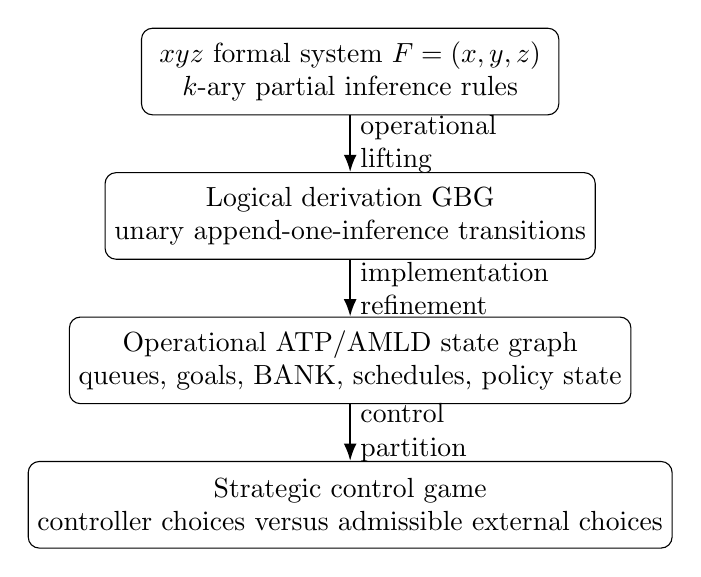
\begin{tikzpicture}[
box/.style={draw,rounded corners,align=center,minimum width=5.3cm,minimum height=1.1cm},
arr/.style={-{Latex[length=2.2mm]},thick},
node distance=0.72cm
]
\node[box] (f) {$xyz$ formal system $F=(x,y,z)$\\$k$-ary partial inference rules};
\node[box,below=of f] (g) {Logical derivation GBG\\unary append-one-inference transitions};
\node[box,below=of g] (o) {Operational ATP/AMLD state graph\\queues, goals, BANK, schedules, policy state};
\node[box,below=of o] (s) {Strategic control game\\controller choices versus admissible external choices};
\draw[arr] (f) -- node[right,align=left]{operational\\lifting} (g);
\draw[arr] (g) -- node[right,align=left]{implementation\\refinement} (o);
\draw[arr] (o) -- node[right,align=left]{control\\partition} (s);
\end{tikzpicture}
\caption{The GBG synthesis has three layers. Statements valid at one layer should not be promoted automatically to another.}
\end{figure}

\section{AMLD global states are already rule-complete candidates}

Version 48 defines a realized global accepted state
\[
X_k=(S_k^P,S_k^R,S_k^D,S_k^I,S_k^C,
B_k^{\rm obj},B_k^{\rm meta},\Pi_k,\Sigma_k,\tau_k).
\]
This tuple is close to what the GBG paper calls a rule-complete state: it records the local accepted states of all five roles, the typed BANK components, provenance, the accepted settlement classes, and first-settlement time.

To turn the AMLD into a literal transition system, one adds whatever finite scheduler and implementation metadata is required to determine the next accepted transitions. A state is then rule-complete relative to the chosen AMLD transition semantics.

\begin{definition}[AMLD transition game]
Fix an AMLD architecture, a finite representation of its accepted operational states, a scheduler policy class, and verifier-gated transition rules. The AMLD transition game is the directed labeled state system whose vertices are rule-complete accepted AMLD states and whose edges are accepted service, certificate, BANK, or settlement transitions permitted by the frozen architecture.
\end{definition}

This use of ``game'' need not imply competition. It means a rule-governed transition system. Strategic analysis enters only after transition authority is partitioned among roles, scheduler, environment, or controller.

\section{Nonstarvation as a strategic admissibility condition}

Version 48 defines a baseline-preserving prover channel and a $P$-nonstarving unit-rate schedule. It then proves the constituent-ATP emulation theorem: if standalone $P_\star$ proves $T$ after $m$ local transitions, the AMLD either settles through another role before global round $m$ or $P$ reproduces the standalone proof by round $m$.

The GBG viewpoint identifies the logical form of this statement.

\begin{definition}[Scheduler-admissible environment]
Fix a prover channel $P$. An environment play is scheduler-admissible through round $m$ if, unless mathematical settlement has already occurred, it grants $P$ at least one baseline local transition opportunity in every global round $1,\ldots,m$.
\end{definition}

\begin{theorem}[Scheduler-robust emulation theorem]
Assume:
\begin{enumerate}[label=(\roman*),leftmargin=2.2em]
\item standalone $P_\star$ reaches a verifier-accepted proof of $T$ after $m$ local transitions from $B_0$;
\item the AMLD prover $P$ is baseline-preserving relative to $P_\star$;
\item every environment play under consideration is scheduler-admissible through round $m$;
\item foreign deposits may be ignored by $P$ for purposes of reproducing the baseline path.
\end{enumerate}
Then every admissible global play either enters some settlement region before round $m$ or enters the $P$-settlement region by round $m$.
\end{theorem}

\begin{proof}
Consider any admissible global play. If another role settles before round $m$, the first alternative holds. Otherwise the play remains unsettled through the preceding rounds. Scheduler admissibility therefore gives $P$ at least $m$ baseline local opportunities by the end of round $m$. Baseline preservation lets $P$ execute the same $m$ local transitions as $P_\star$, ignoring foreign deposits when necessary. The resulting certificate is verifier-accepted, so the play enters the $P$-settlement region by round $m$.
\end{proof}

\begin{remark}[Why the GBG reformulation matters]
The result is stronger in interpretation, not in hypotheses, than the bare phrase ``AMLD can emulate the ATP.'' It says the conclusion survives \emph{every} scheduler behavior inside a declared admissible class. Thus nonstarvation converts an existential baseline route into a robust settlement guarantee against scheduling choices that remain after the constraint is imposed.
\end{remark}

\begin{example}[Starvation destroys the forced horizon]
Suppose $P_\star$ needs exactly two local transitions. If the global scheduler is unconstrained and may forever service only other nonsettling channels, then a two-step proof still exists in the logical derivation graph, but the global forced-settlement horizon for $P$ is infinite. Imposing unit-rate nonstarvation restores the bound of two global rounds, unless another role settles first.
\end{example}

This is the cleanest illustration of
\[
\boxed{H_{\mathrm{proof}}<\infty\quad\text{while}\quad H_{\mathrm{force}}=\infty}
\]
when external scheduling is unconstrained.

\section{BANK growth as conservative road-building}

Version 48 proves the conservative BANK invariant. If every accepted object-level deposit $\lambda$ is certified from the preceding BANK, then
\[
B_k^{\rm obj}\subseteq\Con_F(B_0),
\qquad
\Con_F(B_k^{\rm obj})=\Con_F(B_0).
\]
It also proves the cooperative proof-horizon theorem
\[
\|T\|_F(B_{k+1}^{\rm obj})\le \|T\|_F(B_k^{\rm obj})
\]
for object-level settlement targets under monotone BANK growth.

The GBG interpretation is precise: the set of consequences is unchanged, but the initial resources of the explicit-premise derivation game have improved.

\begin{theorem}[Logical road-building theorem]
Assume $B\subseteq B'\subseteq\Con_F(B)$. For every target $T$,
\[
\Con_F(B')=\Con_F(B),
\]
and
\[
H_F^{\mathrm{inf}}(B',T)\le H_F^{\mathrm{inf}}(B,T).
\]
Thus conservative premise enlargement may shorten the directed distance from the new initial state to $W_T$ without changing whether $W_T$ is reachable at all.
\end{theorem}

\begin{proof}
Since $B'\subseteq\Con_F(B)$, idempotence and monotonicity of consequence closure give
\[
\Con_F(B')\subseteq\Con_F(\Con_F(B))=\Con_F(B).
\]
Since $B\subseteq B'$, monotonicity gives the reverse inclusion. For the horizon inequality, every proof from $B$ is also a proof from $B'$, so minimization over the larger premise set cannot increase the minimum number of inference steps.
\end{proof}

The slogan is therefore not merely metaphorical:
\[
\boxed{\text{same reachable theorem region, potentially shorter explicit route}.}
\]

\subsection{Macro shortcuts versus expanded primitive cost}

Version 48 correctly warns that a deposited lemma may behave as a macro. A one-step proof from the enlarged BANK can expand to a long primitive proof from $B_0$. Thus road-building in the explicit-premise graph need not shorten the fully expanded primitive certificate.

\begin{proposition}[Macro-expansion caution]
There is no general implication
\[
H_F^{\mathrm{inf}}(B',T)<H_F^{\mathrm{inf}}(B,T)
\quad\Longrightarrow\quad
\text{a shorter fully expanded primitive proof of }T\text{ from }B.
\]
\end{proposition}

\begin{proof}
A new premise $\lambda\in B'$ may itself require a long proof from $B$. Treating $\lambda$ as an available premise contracts that proof to zero local cost in the enlarged problem. Expanding the macro restores its derivation and can eliminate the apparent saving.

For a concrete two-rule example, let $B=\{a\}$ and let the primitive rules be
\[
a\longmapsto\lambda,
\qquad
\lambda\longmapsto T.
\]
Then $H_F^{\mathrm{inf}}(B,T)=2$.  After depositing the already proved lemma and taking
$B'=B\cup\{\lambda\}$, one has $H_F^{\mathrm{inf}}(B',T)=1$.  But the one-step proof from $B'$ expands back to the same two primitive inference steps from $B$; no shorter fully expanded primitive proof from $B$ has been produced.
\end{proof}

\section{When BANK also improves a forced horizon}

Ordinary proof-horizon monotonicity requires only premise inclusion. Forced-horizon monotonicity is more delicate because changing the state may also change environment choices.

\begin{theorem}[Conditional robust-horizon monotonicity]
Consider two strategic settlement games on comparable states, before and after a BANK enlargement. Assume:
\begin{enumerate}[label=(\roman*),leftmargin=2.2em]
\item every old controller move remains available after enlargement;
\item BANK enlargement may add controller moves;
\item it does not add new environment moves that can delay settlement;
\item old settlement states remain settlement states; and
\item transition costs are unchanged on old moves.
\end{enumerate}
Then for every state that is forced-settling before enlargement, the post-enlargement forced-settlement horizon is no greater.
\end{theorem}

\begin{proof}
The controller can ignore all new moves and replay its old forcing strategy. By (iii), the environment has no new delaying responses, and by (iv) the old terminal objective remains valid. Therefore the old worst-case bound remains achievable; minimization over the larger controller strategy set can only improve or preserve it.
\end{proof}

\begin{remark}[Why the hypotheses matter]
At the implementation level, extra BANK material can enlarge candidate sets, alter queue order, increase indexing costs, or interact with caps. Version 48 already warns that logical horizon monotonicity does not imply heuristic runtime monotonicity. The same warning prevents an unconditional robust-horizon theorem unless the strategic move sets are controlled explicitly.
\end{remark}

\section{Learned legal-move ranking in GBG language}

Version 48 defines a learned legal-move ranker
\[
s_\theta:\{(S,a):a\in A(S)\}\to\mathbb R
\]
that changes ordering or sampling weight among already legal candidate applications. The verifier remains the trust boundary.

The GBG reformulation is immediate but useful:
\[
\boxed{\text{the ranker changes move selection, not the legal-move relation}.}
\]

\begin{proposition}[Policy/legality separation]
Fix an operational state graph and a sound verifier acceptance relation. Replacing one policy for selecting among legal outgoing actions by another cannot create a new verifier-accepted theorem state outside the formal consequence relation, provided the candidate-generation legality and verifier semantics are unchanged.
\end{proposition}

\begin{proof}
A policy selects which legal transitions to explore and in what order. Every accepted theorem certificate must still consist of legal underlying inference applications and pass the unchanged sound verifier. Search allocation may change hitting time or bounded-budget success but not object-level validity.
\end{proof}

This places learned ATP guidance, A* priorities, Hilbert schedules, proof compasses, novelty bonuses, and related heuristics in one category: \emph{navigation policies over a fixed or conservatively evolving legal transition structure}.

\section{Causal BANK depth and path compression}

Version 48 defines causal BANK depth $\delta(\lambda)$ by recursively expanding accepted deposit certificates and taking the maximum primitive inference depth from original BANK leaves to the deposited formula. This gives a schedule-insensitive dependency quantity.

The GBG synthesis suggests two simultaneous views of a deposited lemma $\lambda$:
\begin{enumerate}[leftmargin=2em]
\item in the expanded primitive graph, $\lambda$ sits at a positive dependency depth from $B_0$;
\item in the post-deposit explicit-premise graph, $\lambda$ is available at the starting boundary and can act as a zero-local-cost resource for later search.
\end{enumerate}

Thus BANK compression is a quotient-like path contraction. It does not erase provenance because the accepted certificate stores the expansion map back to primitive inference structure.

\begin{definition}[Certified path contraction]
A certified path contraction replaces a verified finite derivation subpath from earlier BANK resources to $\lambda$ by direct availability of $\lambda$ in later explicit-premise problems, while retaining a provenance pointer to the accepted expansion certificate.
\end{definition}

This definition separates computational reuse from logical strengthening. The contracted search graph can be dramatically easier to navigate even when the underlying consequence closure is unchanged.

\section{A minimal worked example}

Let
\[
B_0=\{a,b\}
\]
and let $F$ contain primitive rules
\[
r_1(a,b)=c,
\qquad
r_2(c)=d,
\qquad
r_3(b)=e,
\qquad
r_4(e)=d.
\]
The target is $d$.

There are two two-step proofs:
\[
(a,b)\xrightarrow{r_1}c\xrightarrow{r_2}d
\]
and
\[
(a,b)\xrightarrow{r_3}e\xrightarrow{r_4}d.
\]
Hence
\[
H_F^{\mathrm{inf}}(B_0,d)=2.
\]
The derivation history tree has at least two depth-two target histories, while a state representation that remembers only the final fact $d$ would identify their target endpoint. A future-complete representation may still distinguish intermediate states $\{a,b,c\}$ and $\{a,b,e\}$ because their legal continuations differ.

Now suppose the first channel certifies $c$ and deposits it conservatively. Then
\[
B_1=\{a,b,c\}
\]
and
\[